
\section{Newton's 3rd Law, Tension, and Normal Forces\footnote{
1990-93 Dept. of Physics and Astronomy, Dickinson College. Supported by FIPSE
(U.S. Dept. of Ed.) and NSF. Portions of this material may have been modified
locally and may not have been classroom tested at Dickinson College.
}}

\makelabheader %(Space for student name, etc., defined in master.tex or labmanual_formatting_commands.tex)

\textbf{Objectives }

\begin{itemize}
\item To investigate Newton's 3rd law of motion. 
\item To explore the characteristics of two different types of forces: tension
(in strings, ropes, springs, and chains), and normal forces (which support objects
that are in contact with solid surfaces).
\end{itemize}
\textbf{Apparatus} 

\begin{itemize}
\item Spring scales (2) 
\item Variety of masses 
\item Rubber band 
\item Various lengths of string 
\item Pulleys (2)
\end{itemize}
\textbf{An Introduction to Newton's Third Law }

In order to apply Newton's laws to complex situations with strings, pulleys,
inclined planes and so forth, we need to consider a third force law formulated
by Newton having to do with the forces of interaction between two objects. In
order to ``discover'' some simple aspects of the third law,
you should make some straightforward observations using 2 spring scales and
a set of masses.

\vspace{0.3cm}
{\par\centering 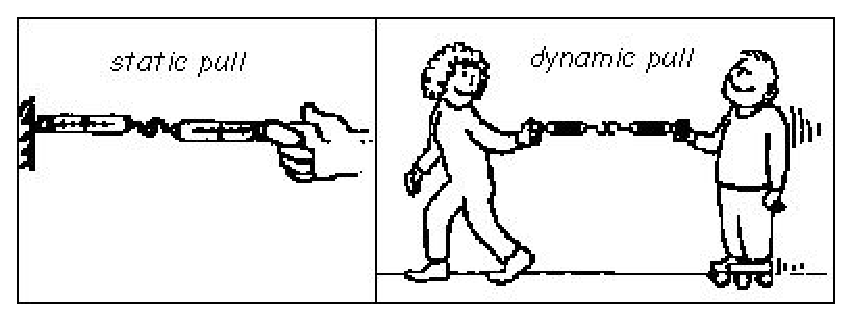
\includegraphics{newton/newton_fig1.eps} \par}
\vspace{0.3cm}

\textbf{Activity 1: Newton's 3rd Law Forces of Interaction }

Set up the situations shown in the diagram above and see if there are any circumstances
in which the object that is pulling and the object that is being pulled exert
different forces on each other. Describe your conclusions below. Note: You can
drag the mass set block across the table for your dynamic observations.
\answerspace{20mm}

\pagebreak[2]
In contemporary English, Newton's third law can be stated as follows:

\textbf{Newton's Third Law }

\textit{If one object exerts a force on a second object, then the second object
exerts a force back on the first object which is equal in magnitude and opposite
in direction to that exerted on it by the first object.}

In mathematical terms, using vector notation, we would say that the forces of
interaction of object 1 on object 2 are related to the forces of interaction
of object 2 on object 1 as follows:

\vspace{0.3cm}
{\par\centering 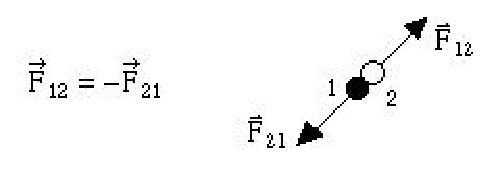
\includegraphics{newton/newton_fig2.eps} \par}
\vspace{0.3cm}

Newton actually formulated the third law by studying the interactions between
objects when they collide. It is difficult to understand the significance of
this law fully without first studying collisions. Thus, we will consider this
law again in the study of collision processes.

\bigskip
\textbf{Tension Forces }

When you pull on one end of a rope attached to a crate, a force is transmitted
down the rope to the crate. If you pull hard enough the crate may begin to slide.
Tension is the name given to forces transmitted in this way along devices that
can stretch such as strings, ropes, rubber bands, springs, and wires.

\vspace{0.5cm}
{\par\centering 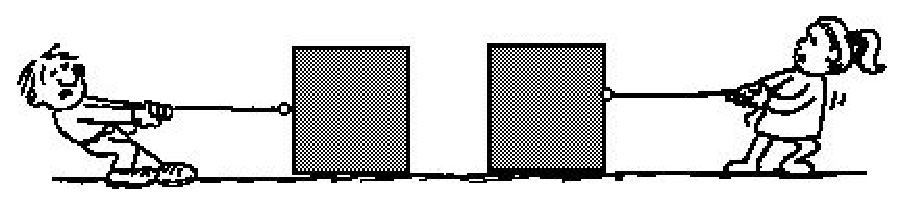
\includegraphics[width=\textwidth]{newton/newton_fig3.eps} \par}
\answerspace{0.5cm}

The end of the rope which is tied to the crate can apply a force to the crate
only if you first pull on the other end of the rope.  

In order
to analyze situations in which objects are attached by strings, rubber bands,
or ropes it is necessary to understand some attributes of tension forces. We
need to answer the following related questions:

\begin{enumerate}
\item (a) What is the mechanism for creating tension in strings, ropes, and rubber
bands? (b) If a string exerts a tension force on an object at one end, what
is the magnitude and direction of the tension force it exerts on another object
at its other end?
\item What happens to the magnitude and directions of the tension forces at each end
of a string and in the middle of that string when the direction of the string
is changed by a post or pulley?
\item Can a flexible force transmitter (like a string) support a lateral (or sideways)
force?
\end{enumerate}

\pagebreak[3]
\textbf{Mechanisms for Tension and the Direction of Forces }

For these observations you should stretch a rubber band and then a string between
your hands as shown in the diagram below. First, just feel the directions of
the forces. Then add the spring scales and both feel and measure the forces.

\vspace{0.3cm}
{\par\centering 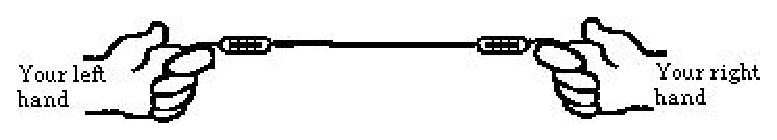
\includegraphics{newton/newton_fig4.eps} \par}
\vspace{0.3cm}

\textbf{Activity 2: Tension Mechanisms \& Force Directions }

(a) Pull on the two ends of a rubber band. (Forget about the spring scales for
now). Does the rubber band stretch? What is the direction of the force applied
by the rubber band on your right hand? On your left hand?
\answerspace{20mm}

(b) Does the magnitude of the forces applied by the rubber band on each hand
feel the same?
\answerspace{20mm}

(c) Repeat this activity with a string instead of a rubber band. This time,
use a spring scale at each end to measure the forces at the ends of the string.
Does the string stretch? (Look carefully!)
\answerspace{20mm}

(d) If you pull by the same amount on the string as you did on the rubber band,
does substituting the string for the rubber band change anything about the directions
and magnitudes of the tension forces exerted on each hand? 
\answerspace{10mm}

(e) If the forces caused by the string on your left and right hands respectively
are given by F\( _{T1} \) and F\( _{T2} \), what is the equation that relates
these two forces?
\answerspace{20mm}

\pagebreak[3]
\textbf{Tension Forces when a String Changes Direction }

Suppose you were to hang equal masses of $m = 0.5$
kg in the various configurations
shown below. Predict and measure the tension in the string for each of the following
situations.

\vspace{0.3cm}
{\par\centering 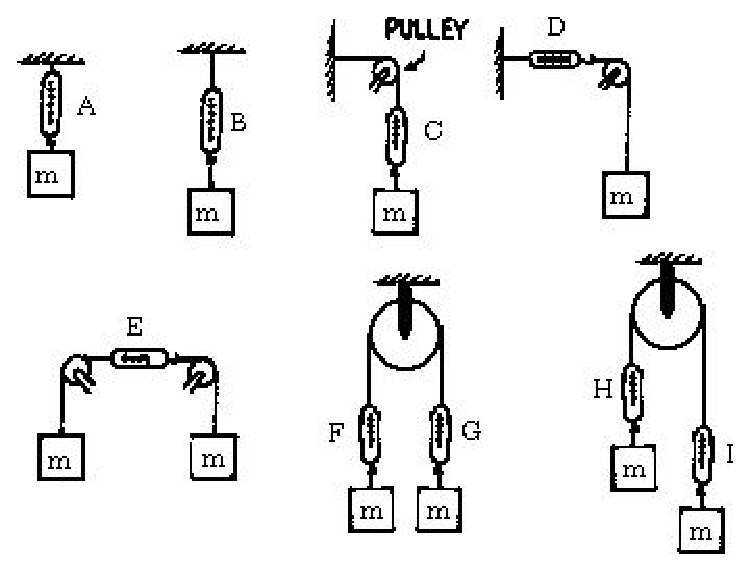
\includegraphics{newton/newton_fig5.eps} \par}
\answerspace{0.5cm}

\textbf{Activity 3: Tension and Direction Changes}

(a) For each configuration shown above, predict the reading in newtons on each
of the spring scales; these readings indicate the forces that are transmitted
by the tensions at various places along the string. Then measure all of the
forces and record their values. Note: Remember that m = 0.5 kg.

\answerspace{0.5cm}
\hfill{}Predicted Force Magnitudes \hfill{}Measured Force Magnitudes\hfill{}

\hfill{}F\( _{A} \) = \rule{1.0in}{0.1pt} N \hfill{}F\( _{A} \) = \rule{1.0in}{0.1pt}
N\hfill{}

\hfill{}F\( _{B} \) = \rule{1.0in}{0.1pt} N \hfill{}F\( _{B} \) = \rule{1.0in}{0.1pt}
N\hfill{}

\hfill{}F\( _{C} \) = \rule{1.0in}{0.1pt} N \hfill{}F\( _{C} \) = \rule{1.0in}{0.1pt}
N\hfill{}

\hfill{}F\( _{D} \) = \rule{1.0in}{0.1pt} N \hfill{}F\( _{D} \) = \rule{1.0in}{0.1pt}
N\hfill{}

\hfill{}F\( _{E} \) = \rule{1.0in}{0.1pt} N \hfill{}F\( _{E} \) = \rule{1.0in}{0.1pt}
N\hfill{}

\hfill{}F\( _{F} \) = \rule{1.0in}{0.1pt} N \hfill{}F\( _{F} \) = \rule{1.0in}{0.1pt}
N\hfill{}

\hfill{}F\( _{G} \) = \rule{1.0in}{0.1pt} N \hfill{}F\( _{G} \) = \rule{1.0in}{0.1pt}
N\hfill{}

\hfill{}F\( _{H} \) = \rule{1.0in}{0.1pt} N \hfill{}F\( _{H} \) = \rule{1.0in}{0.1pt}
N\hfill{}

\hfill{}F\( _{I} \) = \rule{1.0in}{0.1pt} N \hfill{}F\( _{I} \) = \rule{1.0in}{0.1pt}
N\hfill{}
\answerspace{0.5cm}

\pagebreak[3]
(b) Based on Newton's third law and the observations you just made, answer the
following questions using vector notation. If the muscle man in the diagram
below is pulling to the left on a rope with a force of \textbf{F} = -(150 N)\textbf{i}.

\vspace{0.3cm}
{\par\centering 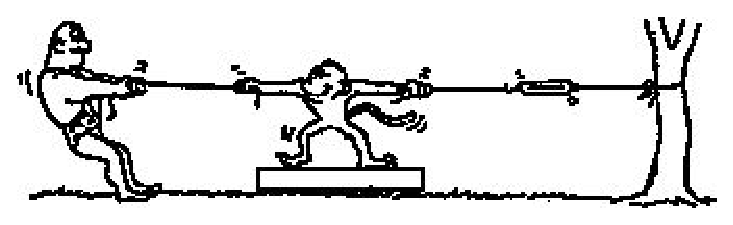
\includegraphics{newton/newton_fig6.eps} \par}
\vspace{0.3cm}

(1) What is the magnitude and direction of the force that the rope is exerting
on the man? \rule{1.0in}{0.1pt}

(2) What force is the left-hand rope exerting on the monkey's right arm? \rule{1.0in}{0.1pt}

(3) What force is the spring scale experiencing on its left end? \rule{1.0in}{0.1pt}

(4) What force is the spring scale experiencing on its right end? \rule{1.0in}{0.1pt}

(5) What is the reading on the spring scale? \rule{1.0in}{0.1pt}

(6) What force is the rope exerting on the tree? \rule{1.0in}{0.1pt}

(7) What force is the tree exerting on the rope? \rule{1.0in}{0.1pt}

(c) Summarize what your observations reveal about the nature of tension forces
everywhere along a string.
\answerspace{20mm}

\textbf{Can a String Support Lateral Forces? }

Take a look at the diagram below. Can the strongest member of your group stretch
a string or rope so that it is perfectly horizontal when a 10 kg mass is hanging
from it? In other words, can the string provide a force that just balances the
force exerted by the mass?

\vspace{0.3cm}
{\par\centering 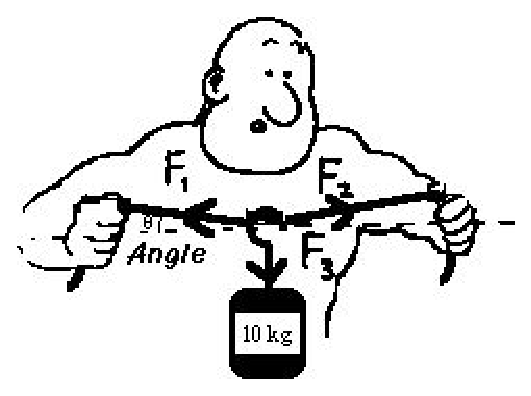
\includegraphics{newton/newton_fig7.eps} \par}
\answerspace{0.5cm}

\pagebreak[2]
\textbf{Activity 4: Can a String Support a Lateral Force?} 

(a) Draw a vector diagram showing the directions of the forces exerted by the
strings on the mass hook in the diagram below. What would happen to the direction
of the forces as \( \theta  \) goes to zero? Do you think it will be possible
to support the mass when \( \theta  \) = 0? Why?

\vspace{0.3cm}
{\par\raggedright 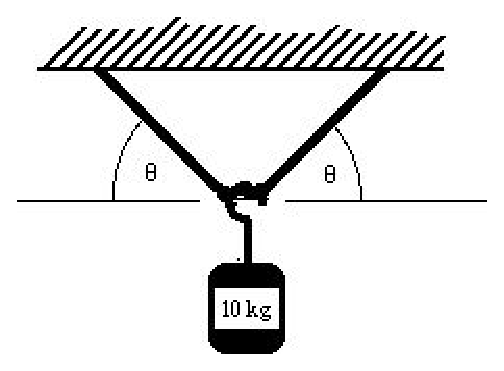
\includegraphics{newton/newton_fig8.eps} \par}
\vspace{0.3cm}

(b) Now, try holding a mass horizontally with a string. Explain why it is not possible to hold the string horizontal.
\answerspace{20mm}

\textbf{Normal Forces} 

A book resting on a table does not move; neither does a person pushing against
a wall. According to Newton's first law the net force on the book and on the
person's hand must be zero. We have to invent another type of force
to explain why books don't fall through tables and hands don't usually punch
through walls. The force exerted by any surface always seems to act in a direction perpendicular to that surface; such a force is known as a normal force (normal meaning perpendicular).

\textbf{Activity 5: Normal Forces }

(a) The diagram below shows a block sliding along a table near the surface of
the earth at a constant velocity. According to Newton's first law, what is the
net force on the block? In other words, what is the vector sum of all the forces on the block?

\vspace{0.3cm}
{\par\raggedright 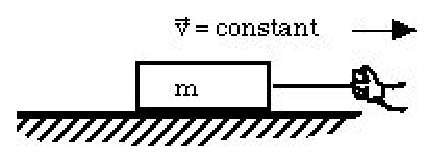
\includegraphics{newton/newton_fig9.eps} \par}
\vspace{0.3cm}

(b) The net force is made up of four forces.  
In what direction does each one act? Draw a
diagram indicating the direction of each of the forces.
\answerspace{20mm}

\pagebreak[2]
\textbf{Gravitational Force on a Mass on an Incline }

Suppose that a block of mass $m$ is perched on an incline of angle \( \theta  \)
as shown in the diagram below. Also suppose that you know the angle of the incline
and the magnitude and direction of the gravitational force vector. What do you
predict the magnitude of the component of the force vector will be parallel
to the plane? Perpendicular to the plane?

\vspace{0.3cm}
{\par\centering 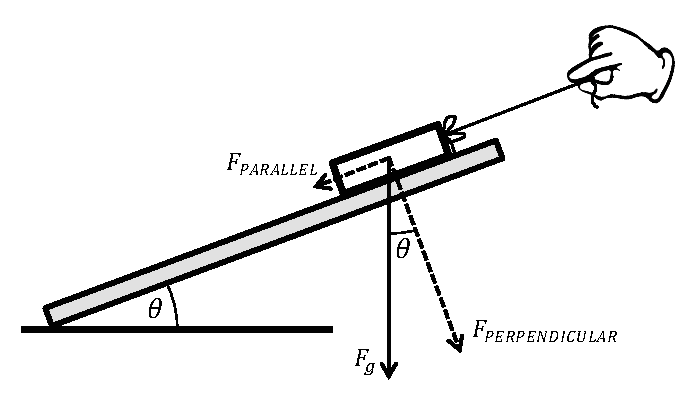
\includegraphics{newton/newton_fig10_new.eps} \par}
\vspace{0.3cm}

\textbf{Activity 6: Components of F\( _{g} \) on an Incline }

(a) The angle that the incline makes with the horizontal and the angle between
\( {\bf F}_{{\mbox{\small perpendicular}}} \) and F\( _{g} \) are the same. Explain why.
\vspace{20mm}

(b) Choose a coordinate system with the x-axis parallel to the plane with the
positive direction up the plane. Using normal mathematical techniques for finding the components of a vector, find the values of 
\( F_{\mbox{\small parallel}} \) and \( F_{\mbox{\small perpendicular}} \)
as a function of \( F_{g} \) and the angle of the incline \( \theta  \).
\vspace{20mm}

(c) Find an equation for the magnitude of the normal force exerted on the
block by the surface of the incline. Hint: Use Newton's first law and the knowledge that the block is not moving in a direction perpendicular to the plane.

